\documentclass[border=12pt]{standalone}
\def\pgfsysdriver{pgfsys-dvisvgm.def}
\usepackage[dvisvgm]{xcolor}
\usepackage{xeCJK}
\setCJKmainfont{HaranoAjiGothic-Regular.otf}[BoldFont=HaranoAjiGothic-Bold.otf]
\setCJKsansfont{HaranoAjiGothic-Regular.otf}[BoldFont=HaranoAjiGothic-Bold.otf]
\usepackage{amsmath,amssymb,tikz,lmodern}
\usetikzlibrary{arrows.meta,positioning,calc,fit,backgrounds}
\renewcommand{\familydefault}{\sfdefault}
\definecolor{ink}{HTML}{25322F}
\definecolor{green}{HTML}{246657}
\definecolor{tint}{HTML}{EEF4F0}
\definecolor{soft}{HTML}{C6D2CC}
\definecolor{muted}{HTML}{52615B}
\newif\ifJapanese
\newcommand{\Tx}[2]{\ifJapanese #1\else #2\fi}
\newcommand{\Eff}{\overline{\operatorname{Eff}}}
\newcommand{\heading}[3]{{\color{green}\bfseries #1\quad\Tx{#2}{#3}}\\[5pt]}
% A white rectangle makes the complete citation label clickable, including spaces.
\newcommand{\refurl}[2]{\special{dvisvgm:raw <a xlink:href="#1" target="_blank" rel="noopener noreferrer">}{\setlength{\fboxsep}{0pt}\colorbox{white}{\color{green}\underline{\strut #2}}}\special{dvisvgm:raw </a>}}
\tikzset{
 card/.style={draw=soft,fill=white,rounded corners=2pt,align=left,text=ink,font=\fontsize{10.5}{14}\selectfont,inner xsep=12pt,inner ysep=10pt,text width=16cm},
 half/.style={card,text width=7.1cm,minimum height=2.05cm},
 result/.style={draw=green,fill=tint,line width=.9pt},
 reason/.style={align=left,text=muted,font=\fontsize{9}{12}\selectfont,inner sep=0pt,text width=14.3cm},
 branchreason/.style={reason,text width=6.4cm},
 edge/.style={-{Stealth[length=2.4mm]},draw=green,line width=1pt},
 wire/.style={draw=green,line width=1pt},
}
% Keep the arrow in a dedicated left gutter; explanations never cover it.
\newcommand{\flow}[3]{
 \coordinate (#2-from) at ($(#1.south)+(-7.7,0)$);
 \coordinate (#2-to) at ($(#2.north)+(-7.7,0)$);
 \draw[edge] (#2-from)--(#2-to);
 \node[reason,anchor=west] (#2-reason) at ($(#2-from)!.5!(#2-to)+(.55,0)$) {#3};
}

\newcommand{\RA}[1]{\refurl{\sourceRA}{#1}}
\newcommand{\OI}[1]{\refurl{\sourceOI}{#1}}
\newcommand{\FF}[1]{\refurl{\sourceFF}{#1}}
\newcommand{\FFcor}[1]{\refurl{\sourceFFcor}{#1}}
\newcommand{\BBT}[1]{\refurl{\sourceBBT}{#1}}
\newcommand{\FG}[1]{\refurl{\sourceFG}{#1}}
\newcommand{\CP}[1]{\refurl{\sourceCP}{#1}}
\newcommand{\BDPP}[1]{\refurl{\sourceBDPP}{#1}}
\newcommand{\pe}{\mathrel{\geq_{\mathrm{pe}}}}
\newcommand{\rowflow}[3]{
 \coordinate (#2-a) at ($(#1.south)+(-3.45,0)$);
 \coordinate (#2-b) at ($(#2.north)+(-3.45,0)$);
 \draw[edge] (#2-a)--(#2-b);
 \node[branchreason,anchor=west] at ($(#2-a)!.5!(#2-b)+(.45,0)$) {#3};
}

\newcommand{\sourceRA}{https://github.com/openai/math/blob/fd4aeeb2ee4fc729c18d98444fed42fd0529eeeb/preprints/The-reverse-logarithmic-Kodaira-inequality-and-additivity-September-26-2026/paper.pdf}
\newcommand{\sourceOI}{https://github.com/openai/math/blob/fd4aeeb2ee4fc729c18d98444fed42fd0529eeeb/preprints/Orbifold-and-logarithmic-Iitaka-subadditivity-September-26-2026/paper.pdf}
\newcommand{\sourceFF}{https://www.math.kyoto-u.ac.jp/~fujino/vmhs-sp108.pdf}
\newcommand{\sourceFFcor}{https://www.math.kyoto-u.ac.jp/~fujino/fujino-fujisawa-memo2.pdf}
\newcommand{\sourceBBT}{https://arxiv.org/pdf/1811.12230v3}
\newcommand{\sourceFG}{https://www.numdam.org/item/10.5802/aif.2894.pdf}
\newcommand{\sourceCP}{https://arxiv.org/pdf/1508.02456v4}
\newcommand{\sourceBDPP}{https://arxiv.org/pdf/math/0405285v1}
\Japanesetrue
\begin{document}
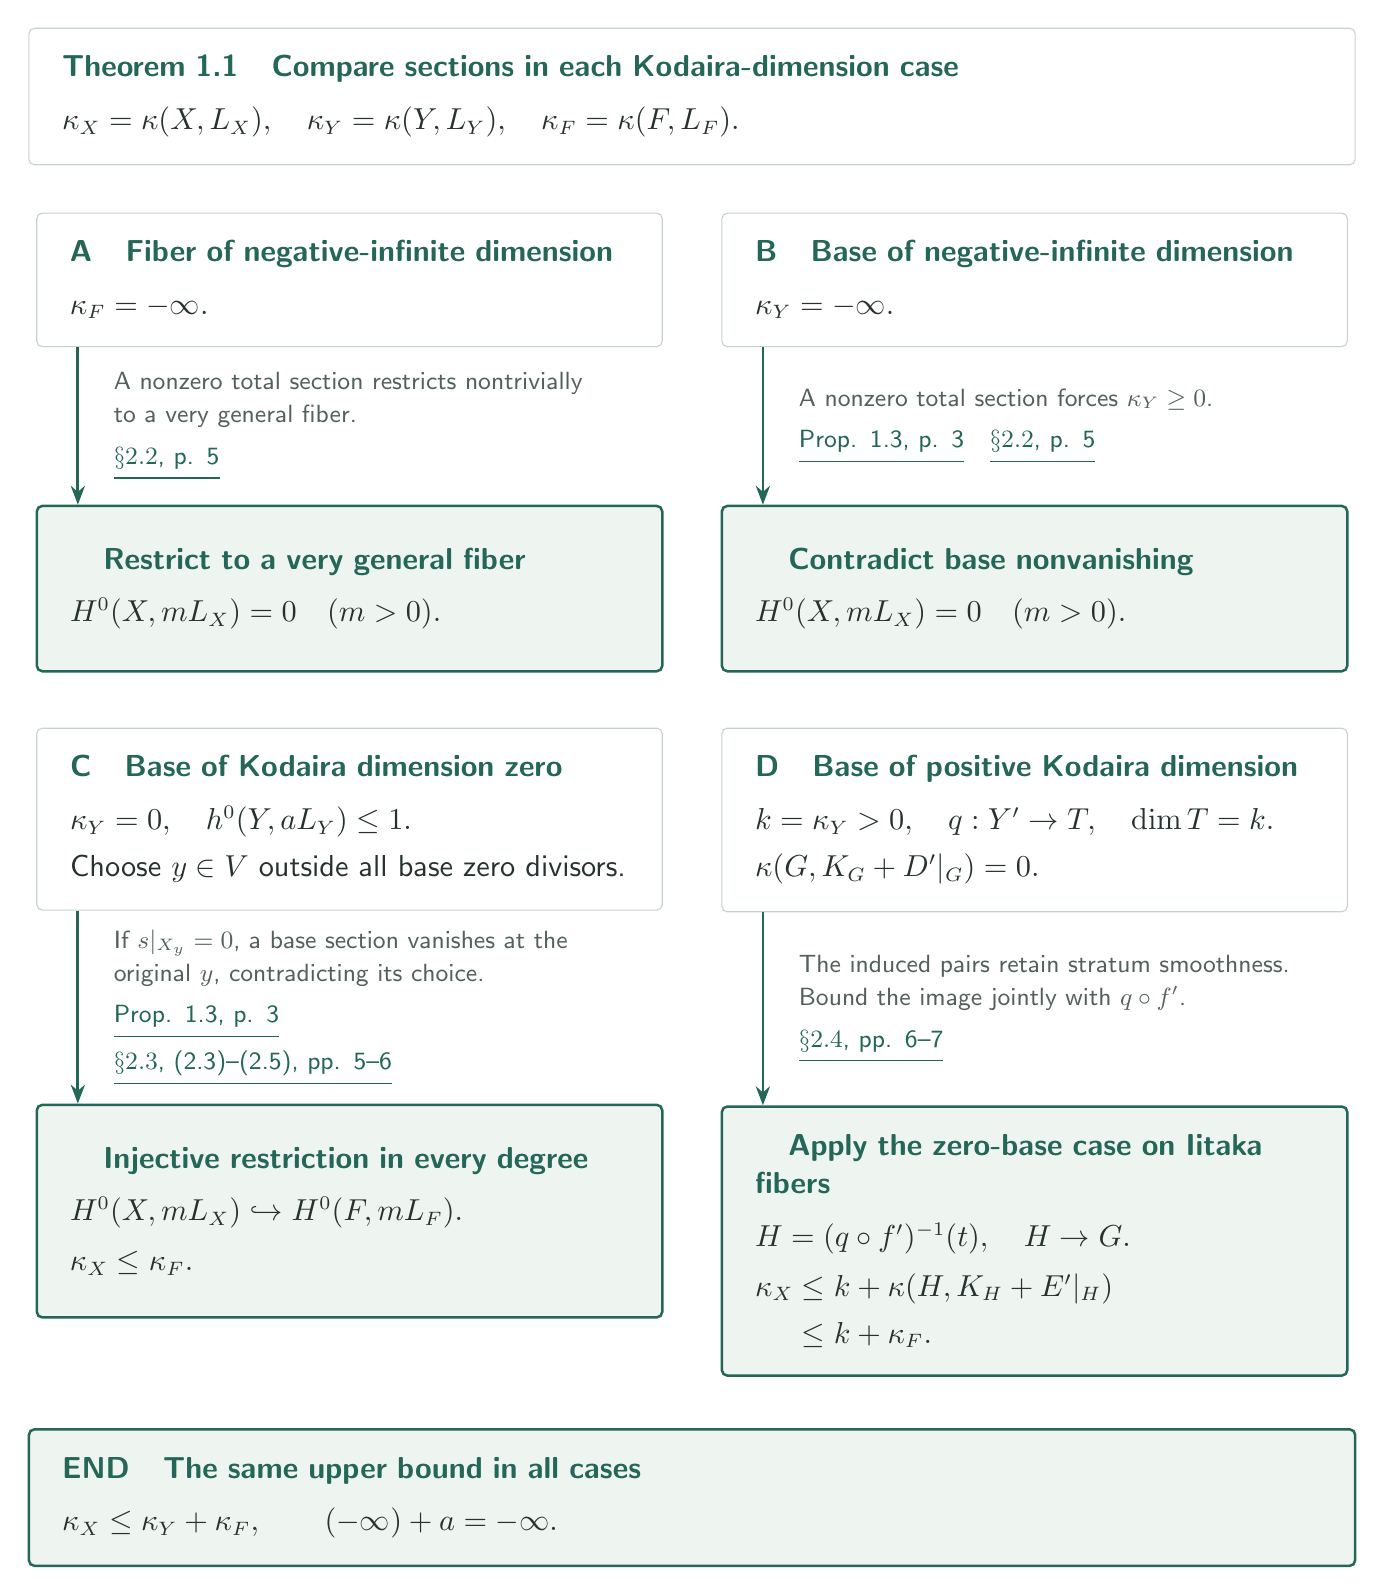
\begin{tikzpicture}
\node[card] (head) {\heading{Theorem 1.1}{小平次元の各場合を切断で比較する}{Compare sections in each Kodaira-dimension case}
$\kappa_X=\kappa(X,L_X),\quad\kappa_Y=\kappa(Y,L_Y),\quad\kappa_F=\kappa(F,L_F).$};
\node[half,below=0.6cm of head.south,anchor=north,xshift=-4.35cm,minimum height=1.6cm] (fn) {\heading{A}{ファイバーが負の無限大}{Fiber of negative-infinite dimension}
$\kappa_F=-\infty.$};
\node[half,below=0.6cm of head.south,anchor=north,xshift=4.35cm,minimum height=1.6cm] (yn) {\heading{B}{底が負の無限大}{Base of negative-infinite dimension}
$\kappa_Y=-\infty.$};
\node[half,result,below=2cm of fn,minimum height=2.1cm] (fnend) {\heading{}{非常に一般のファイバーへ制限}{Restrict to a very general fiber}
$H^0(X,mL_X)=0\quad(m>0).$};
\node[half,result,below=2cm of yn,minimum height=2.1cm] (ynend) {\heading{}{底の非消滅との矛盾}{Contradict base nonvanishing}
$H^0(X,mL_X)=0\quad(m>0).$};
\rowflow{fn}{fnend}{\Tx{非零の全空間切断なら、非常に一般の\\ファイバー上にも非零切断が得られる。}{A nonzero total section restricts nontrivially\\to a very general fiber.}\\[3pt]\RA{$\S2.2$, p. 5}}
\rowflow{yn}{ynend}{\Tx{非零の全空間切断から $\kappa_Y\geq0$。}{A nonzero total section forces $\kappa_Y\geq0$.}\\[3pt]\RA{Prop. 1.3, p. 3}\quad\RA{$\S2.2$, p. 5}}
\node[half,below=0.7cm of fnend,minimum height=1.9cm] (yz) {\heading{C}{底の小平次元0}{Base of Kodaira dimension zero}
$\kappa_Y=0,\quad h^0(Y,aL_Y)\leq1.$\\[3pt]
\Tx{全ての底切断の零因子を避ける $y\in V$。}{Choose $y\in V$ outside all base zero divisors.}};
\node[half,below=0.7cm of ynend,minimum height=1.9cm] (yp) {\heading{D}{正の小平次元の底}{Base of positive Kodaira dimension}
$k=\kappa_Y>0,\quad q:Y'\to T,\quad\dim T=k.$\\[3pt]
$\kappa(G,K_G+D'|_G)=0.$};
\node[half,result,below=2.45cm of yz,minimum height=2.7cm] (yzend) {\heading{}{全次数での制限の単射性}{Injective restriction in every degree}
$H^0(X,mL_X)\hookrightarrow H^0(F,mL_F).$\\[4pt]
$\kappa_X\leq\kappa_F.$};
\node[half,result,below=2.45cm of yp,minimum height=2.7cm] (ypend) {\heading{}{飯高ファイバーで前段を使う}{Apply the zero-base case on Iitaka fibers}
$H=(q\circ f')^{-1}(t),\quad H\to G.$\\[4pt]
$\kappa_X\leq k+\kappa(H,K_H+E'|_H)$\\[3pt]
$\phantom{\kappa_X}\leq k+\kappa_F.$};
\rowflow{yz}{yzend}{\Tx{$s|_{X_y}=0$ なら、元の $y$ で消える\\底切断を作り、点の選択に矛盾する。}{If $s|_{X_y}=0$, a base section vanishes at the\\original $y$, contradicting its choice.}\\[3pt]\RA{Prop. 1.3, p. 3}\\[2pt]\RA{$\S2.3$, (2.3)--(2.5), pp. 5--6}}
\rowflow{yp}{ypend}{\Tx{誘導対はstratumの滑らかさを保つ。\\線形系と $q\circ f'$ の合成像の次元を評価。}{The induced pairs retain stratum smoothness.\\Bound the image jointly with $q\circ f'$.}\\[3pt]\RA{$\S2.4$, pp. 6--7}}
\node[card,result,below=.65cm of ypend.south,anchor=north,xshift=-4.35cm] (end) {\heading{END}{全ての場合で同じ上界}{The same upper bound in all cases}
$\kappa_X\leq\kappa_Y+\kappa_F,\qquad (-\infty)+a=-\infty.$};
\end{tikzpicture}

\end{document}
